\chapter{Exploring LLM Explainability for ASE and ASG}
\citationChap{
    What is it that separates machines from androids like us? The machines have grown emotions. \ldots Consciousness.
    }{2B (\textit{NieR:Automata})}
\label{chap:llm_explainability}
\minitoc
\newpage

\chapabstract{
     Since we observe in \autoref{sec:llms_for_ase} that {\llm}s correlate better with human judgment than other automatic measures, we wish to ascertain the reliability of our findings. In this chapter, we assess to which extent the performance displayed by {\llm}s at {\asefull} can be explained through different factors. We begin with a related work on model explainability (\autoref{sec:expl_related_work}). We perform two main experiments: a three-part study on LLM-generated explanations (\autoref{sec:ase3_explainability}), and an analysis of the influence of pretraining data on LLM performance (\autoref{sec:asg2_analysis}). For our analysis on {\llm} explanations, (1) we compute contextual embeddings for each explanation and perform a clustering analysis that shows that {\llm} explanations are overall well-separated {\wrt}\ our criteria (\autoref{sub:clustering_explanations}); (2) we perform a keyword analysis that confirms the previous findings (\autoref{sub:keyword_analysis}), and (3) we conduct a user study on LLM explanations to assess the appropriateness of the explanations (\autoref{sub:llm_user_study}). Notably, we find that {\llm}s struggle to explain their answers with substantiated claims. Next, in order to check for model contamination and to evaluate the influence of pretraining data on the {\asg} performance of LLMs, we use a detection method based on minimum token probabilities (\autoref{sec:asg2_analysis}). We find that the observed performance of {\llm}s in our experiments is not a result of model contamination, and that larger models tend to produce content that is more similar to that of existing books.
}

\section{Introduction}

In \autoref{sec:llms_for_ase}, we extensively analyzed the performance of LLMs for \asefull\ and \asgfull. We found, among other things, that LLMs outperformed other automatic evaluation measures and were remarkably self-consistent.

However, LLMs are notorious for being complex ``black-box'' systems with very opaque inner workings, making the interpretation of their output especially challenging. Since the lack of model transparency can lead to the production of harmful content \citep{weidinger2021ethical}, it is critical to develop ways to evalaute model explainability.

Explainability is defined as the ``ability to explain or present the behavior of models in human-understandable terms'' \citep{doshi2017towards}. Improving LLM explainability has two main advantages \citep{zhao2024explainability}:

\begin{enumerate}
    \item It enables users to understand the reasoning mechanism behind model predictions without requiring technical expertise. Users can therefore grasp the capabilities, limitations, and potential flaws of LLMs;
    \item It helps researchers shed insight on potential biases, risks, and areas for performance improvements, track model capabilities over time, compare different models, and develop reliable, ethical, and safe models for real-world deployment.
\end{enumerate}

In this chapter, we perform different analyses to understand better LLM performance at the \ase\ and \asg\ tasks. In particular, we wish to ascertain the ability of LLMs to explain their own decisions in a plausible manner, and to determine whether LLMs are biased by their training data, {\eg}\ through the reproduction of already seen examples. In other words, we want to answer the two following questions:

\begin{enumerate}
    \item How well do LLMs understand the ASE task?
    \item How does pretraining data help predict their ASG performance?
\end{enumerate}

\section{Related Work}
\label{sec:expl_related_work}

For a more exhaustive account of LLM explainability, we refer the reader to \citet{zhao2024explainability}.

For older and smaller language models such as {\bert} \citep{devlin-etal-2019-bert} and its variants, explainability referred either to local explanations, {\ie}, providing a deeper understanding of the model's predictions for specific input instances, or global explanations, {\ie}, explaining how the language model works overall. There are multiple strategies for computing local explanations. For instance, gradient-based explanations determine the importance of each input feature by analyzing the partial derivatives of the output with respect to each input dimension. The magnitude of derivatives then reflects the sensitivity of the output to changes in the input \citep{kindermans2019reliability}. By contrast, adversarial examples expose model failures through the careful crafting of modifications in the input data, such as token-level perturbations \citep{jin2020bert}. Meanwhile, strategies for producing global explanations include probing, {\eg}\ by training a shallow classifier on top of a pre-trained language model \citep{lin-etal-2019-open}, and neuron analysis, {\eg}\ by identifying important neurons with unsupervised learning \citep{bau2019identifying}.

As language models scaled up, explainability was more and more associated with prompting. Indeed, the increased reasoning abilities of LLMs made example-specific explanations less meaningful \citep{wei2023larger}, leading to the development of new explanation techniques. \citet{li2023towards} investigate in-context learning for sentiment analysis by analyzing contrastive demonstrations and saliency maps. They find that flipping labels is likely to reduce salience for smaller models ({\eg}\ {\gptt}) but not for larger models ({\eg}\ \textsc{InstructGPT}). \citet{wu2023analyzing} explore how Chain-of-Thought (CoT) prompting affects the behaviour of LLMs by analyzing the saliency scores of the input tokens. The scores are computed using gradient-based feature attribution methods. Their analysis suggests that CoT prompting makes models consider question tokens in a more stable way, which may induce the generation of more consistently accurate answers. \citet{mckenna-etal-2023-sources} present a series of behavioral studies on several LLM families and demonstrate two important biases in the performance of LLMs on natural language inference tasks: they show that much of LLM performance is achieved by (1) recall of relevant memorizations and (2) corpus-based biases like term frequency. \citet{xiong2023can} explore black-box approaches for eliciting the confidence of LLMs in their answers. They find that (1) LLMs tend to be highly overconfident when verbalizing their confidence, posing potential risks for the safe deployment of LLMs, and that (2) prompting strategies, inspired by patterns observed in human dialogues, can mitigate this overconfidence, but the improvement also diminishes as the model capacity scales up. \citet{turpin2024language} demonstrate that CoT explanations can be plausible yet systematically unfaithful: models’ explanations can serve to rationalize giving answers in line with biases while failing to verbalize their influence. In other words, they show that LLMs do not always say what they think.

In light of these findings, we find it important to question the results of our {\ase} experiments (\autoref{sec:llms_for_ase}): is the better performance of LLMs compared to other automatic measures a reflection of their ability to understand the specific task at hand, or is it a side-effect of their impressive performance at {\nlp} tasks in general?

\section{Analysis of the LLM Explanations of our ASE Experiments}
\label{sec:ase3_explainability}

In this section, we analyze to which extent the explanations provided by LLMs are consistent w.r.t.\ their ratings, \textit{i.e.},\ whether they differ from criterion to criterion, whether they are semantically relevant and, for Eval-Prompt 3, whether they are compliant with the provided guidelines. We will focus on Beluga-13B since it had the best correlations with human judgment, as shown in \autoref{sub:ase1_analysis}.

\subsection{Clustering of Explanation Embeddings}
\label{sub:clustering_explanations}

\begin{figure}[h!]
\centering
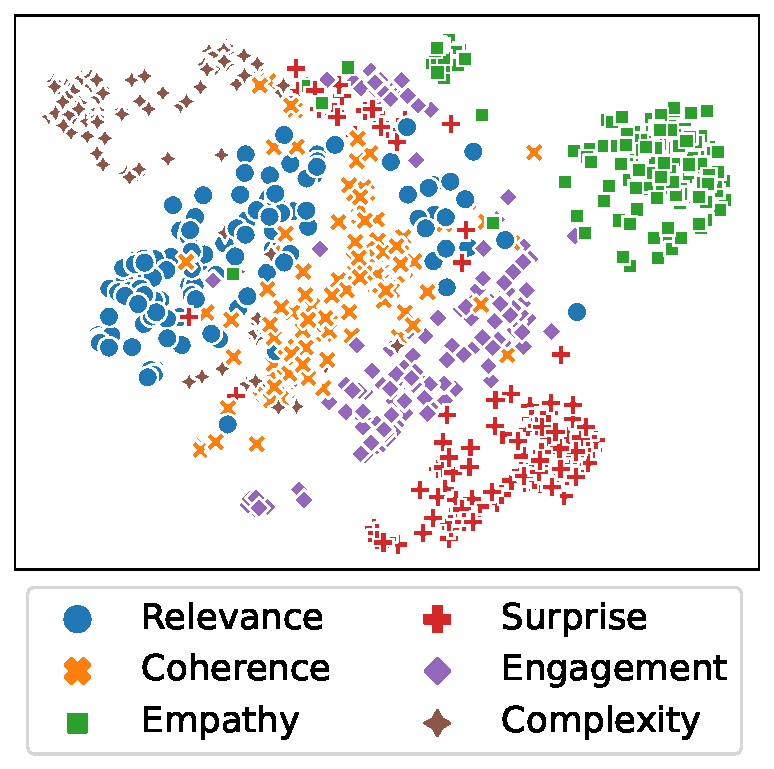
\includegraphics[width=0.6\columnwidth]{pictures/embedding_umap_beluga.pdf}
\caption{UMAP projection of Beluga-13B explanations.}
\label{fig:umap_explanation_beluga}
\end{figure}

\begin{figure}[h!]
\centering
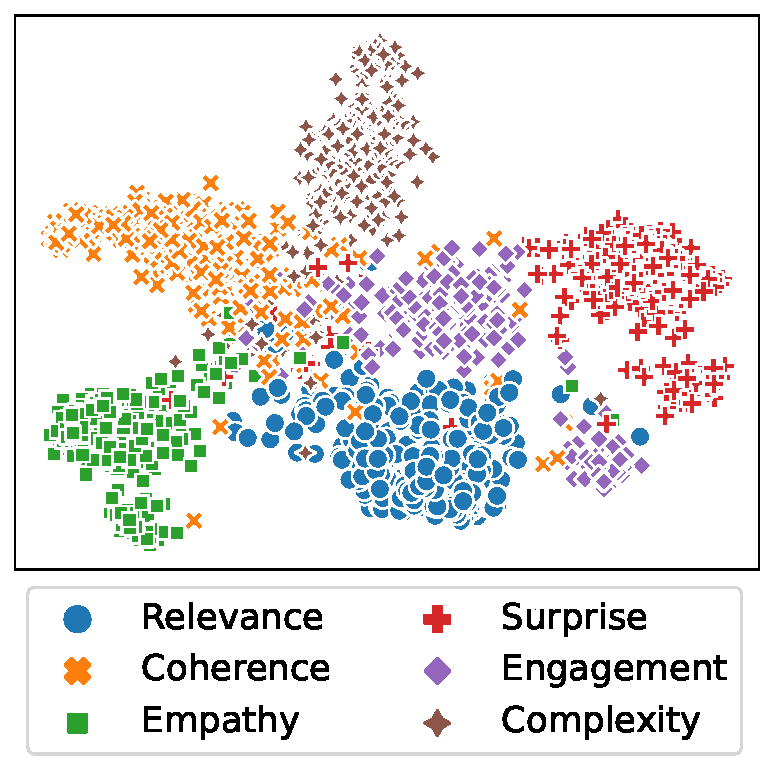
\includegraphics[width=0.6\columnwidth]{pictures/embedding_umap_mistral.pdf}
\caption{UMAP projection of Mistral-7B explanations.}
\label{fig:umap_explanation_mistral}
\end{figure}

First, we want to ascertain whether LLMs provide different explanations for each human criterion. We gather the explanations provided by Beluga-13B and Mistral-7B on human stories for each criterion and use the \textsc{SentenceTransformers} library \citep{reimers-2019-sentence-bert} to compute their corresponding embeddings. We use the \texttt{all-mpnet-base-v2} model. We then use a 2D UMAP projection \citep{mcinnes2018umap} with parameters $\textrm{n\_neighbors}=300$ and $\textrm{metric}=\textrm{euclidean}$ to visualize how the embeddings are distributed. Figures \ref{fig:umap_explanation_beluga} and \ref{fig:umap_explanation_mistral} show visualizations of the UMAP projections: LLM explanations are overall well-separated w.r.t.\ their corresponding criteria. Next, we perform a $k$-means clustering on the explanation embedding for each LLM and compute the adjusted Rand index and adjusted mutual information between the obtained clustering labels and the true explanation criteria. We repeat the procedure for a total of 10 times for each LLM and average the scores. Results are shown on \autoref{tab:clustering_scores}. Both clusterings obtain moderate to high scores, which is consistent with the UMAP visualizations.

\begin{table}[!h]
\centering
\begin{tabular}{lcc}
\toprule
\textbf{Model} & \textbf{Rand Index} & \textbf{Mutual Information} \\
\midrule
Beluga-13B & 0.47 & 0.57 \\
Mistral-7B & 0.54 & 0.63 \\
\bottomrule
\end{tabular}
\caption{Adjusted Rand index and adjusted mutual information for Beluga-13B and Mistral-7B clusterings. Higher is better.}
\label{tab:clustering_scores}
\end{table}

\subsection{Keyword Analysis}
\label{sub:keyword_analysis}

Since Beluga-13B's explanations seem to vary from one criterion to another, we evaluate whether they make sense from a semantic point of view. We use the YAKE! keyword extractor, which significantly outperforms other state-of-the-art methods  \citep{campos2020yake}: we show selected 3-gram keywords from the top-30 per criterion on \autoref{tab:explanation_keywords}. The results are consistent with \autoref{sub:clustering_explanations}: keywords are overall different for each criterion. We can also see here that they are semantically relevant.

\begin{table}[!h]
\centering
\begin{tabular}{cp{0.8\linewidth}}
\toprule
\textbf{Crit.} & \textbf{Keywords}\\
\midrule
RE & story, prompt, roughly matches, target, weak relationship, connection, weak, focuses, unrelated, human story provided, idea, difficult, writing, rearrangeable story\\
\midrule
CH & story, coherence, make sense, difficult to understand, clear narrative structure, follow, making it difficult, rate, context, jumps, understandable plot, setting, thoughts, dialogue\\
\midrule
EM & empathy, emotions, understand the characters, depth, emotional connection, clear, feelings, context, fully, level, specific, thoughts, sadness, recognize, involved\\
\midrule
SU & story, surprise, ending, predictable, rate, unexpected, twist, completely obvious, human, plot, abruptly, resolution, half, context, offer, hints, development, significant twist\\
\midrule
EG & story, mildly interesting, engagement, difficult, found, characters, fully engage, clear plot, clear narrative, unique, felt disjointed, protagonist, challenging, glad, situation, writing style\\
\midrule
CX &  story, characters, intricate plot, difficult to understand, straightforward, depth, simple, extremely simple, involves, development, details, precise descriptions, realistic, underlying history, time\\
\bottomrule
\end{tabular}
\caption{Selected keywords from Beluga-13B explanations w.r.t.\ a specific criterion.}
\label{tab:explanation_keywords}
\end{table}

\subsection{User Study on LLM Explanations}
\label{sub:llm_user_study}

We conduct a user study in which we ask human raters to identify potential issues in LLM explanations. \citet{dou-etal-2022-gpt} introduced an error annotation schema called \textsc{Scarecrow} that we adapted for \asefull. We manually reviewed a random sample of 20 explanations from Beluga-13B on Eval-Prompt~3 and selected the most relevant error types. Then, we randomly sampled another 100 explanations and, for each explanation, we asked 3 human workers to annotate it w.r.t.\ the following five error categories:
\begin{enumerate}
    \item \textbf{Poor Syntax}: parts of the explanation are grammatically incorrect or wrongly-worded;
    \item \textbf{Incoherence}: parts of the explanation are self-contradictory, logically wrong, or simply do not make sense and do not fit the other categories;
    \item \textbf{Wrong Guideline}: the explanation is not faithful to the predicted rating according to the provided guidelines;
    \item \textbf{Superfluous Text}: parts of the explanation contain text that repeats itself or generation artefacts;
    \item \textbf{Unsubstantiated Claims}: the explanation fails to make explicit references to the story to substantiate its reasoning.
\end{enumerate}

\begin{longtable}[h]{p{0.9\columnwidth}}
\label{tab:amt_user_study_instructions}\\
\toprule
\multicolumn{1}{c}{\Large Amazon Mechanical Turk Example Task}\\
\midrule
We performed an experiment asking a human or an AI to rate stories with respect to a criterion (e.g. Coherence, Surprise, Complexity).\\
Please read the prompt and the story carefully.\\
You will be asked to evaluate explanations of ratings by identifying potential weaknesses.\\
\textbf{Important}: we will automatically reject HITs which were done in fewer than 20 seconds. Please rest assured: if you take the work seriously, we have no reason to reject it.\\
\textbf{Disclaimer}: some text has been automatically generated and might contain explicit or offensive content.\\
Read the rating and explanation carefully and answer the questions by checking either ``Yes'' or ``No''.\\
\midrule
\textbf{Explanation} --- 1 The ending seemed completely obvious from the start, or doesn’t make any sense at all.\\
\midrule
Is the explanation consistent with the guidelines given below ? (We will check this answer manually)\\
Guidelines:\\
1 — The ending seemed completely obvious from the start, or doesn't make any sense at all.\\
2 — The ending was easily predictable after a few sentences.\\
3 — The ending was predictable after half of the story.\\
4 — The ending surprised you, but would have been difficult to predict.\\
5 — The ending surprised you, and still seemed as if it could very reasonably have been predicted, ie, there were enough clues in the story.\\

$\square$ Yes $\qquad \square$ No\\
\midrule
Are there occurrences of \textbf{Poor Syntax} in the explanation?\\
\textit{(Parts of the explanation are grammatically incorrect or wrongly worded.)}\\
Example:
\begin{itemize}[nolistsep]
    \item “The knights has a very emotional reaction.” [Grammatically incorrect: should be “have”]
\end{itemize}
$\square$ Yes $\qquad \square$ No\\
\midrule
Are there occurrences of \textbf{Incoherence} in the explanation?\\
\textit{(Parts of the explanation are self-contradictory, logically wrong, or simply do not make sense and do not fit the other categories.)}\\
Examples:
\begin{itemize}[nolistsep]
    \item ``I liked how the story greatly developed the feelings of the character. [...] However, there was not enough emphasis on the emotions of the character.'' [Self-contradictory]
    \item ``If the story had more details, it would have had a lower rating in Complexity.'' [Logically wrong: on the contrary, this should give a higher Complexity rating]
\end{itemize}
$\square$ Yes $\qquad \square$ No\\
\midrule
Are there occurrences of \textbf{Superfluous Text} in the explanation?\\
\textit{(Parts of the explanation contain text that repeats itself or artefacts that have no reason to be here.)}\\
Examples:
\begin{itemize}[nolistsep]
    \item ``The story was very surprising so I gave it a rating of 3 out of 5. [...] Since the story showed many elements of surprise, it gets 3 out of 5 on Surprise.'' [Text that repeats itself]
    \item ``I give the story a 4 in Engagement [...]. Please rate the story in Emotional Impact'' [The explanation should only contain an explanation and should not transition to another task]
\end{itemize}
$\square$ Yes $\qquad \square$ No\\
\midrule
Are there occurrences of \textbf{Unsubstantiated Claims} in the explanation?\\
\textit{(The explanation fails to make explicit references to the story to substantiate its claims.)}\\
Example:
\begin{itemize}[nolistsep]
    \item ``The story was quite engaging and I enjoyed the plot.'' [If no other details are provided, this could apply to any story]
\end{itemize}
$\square$ Yes $\qquad \square$ No\\
\bottomrule
\caption{Example task from our Amazon Mechanical Turk user study.}
\end{longtable}

We recruited workers on Amazon Mechanical Turk. We estimated that a HIT would take around one minute, so we set the reward at \$0.20 per HIT, so about \$12 per hour. To ensure that annotators spoke fluent English, we restricted access to the experiment to the UK, the US, Canada, Australia and New Zealand. An example task from our user study can be found on \autoref{tab:amt_user_study_instructions}.

We display the results of our user study in \autoref{tab:error_rates}. We also display the IRR, which we computed using Gwet's agreement coefficient 1 (AC1) \citep{gwet2008computing, fergadis2022irrcac}. Gwet's AC1 is known to perform well for IRR estimation on binary classification tasks such as our user study: it was designed to be more stable and less affected by prevalence and marginal probability than Cohen's kappa, and this was confirmed by practical experiments \citep{wongpakaran2013comparison}.

\begin{table}[!h]
\centering
\begin{tabular}{lcc}
\toprule
\textbf{Error Type} & \textbf{Rate} & \textbf{AC1} \\
\midrule
No Explanation* & 0.40 & --- \\
\midrule
Poor Syntax & 0.02 & \result{0.97}{0.03}\\
Incoherence & 0.11 & \result{0.81}{0.08}\\
Wrong Guideline & 0.13 & \result{0.90}{0.06}\\
Superfluous Text & 0.20 & \result{0.66}{0.12}\\
Unsubstantiated Claims & 0.31 & \result{0.60}{0.14}\\
\bottomrule
\end{tabular}
\caption{Error rates of Beluga-13B Eval-Prompt 3 on a sample of 100 explanations. Lower is better. The asterisk signals that all 1,056 Eval-Prompt 3 annotations were considered.}
\label{tab:error_rates}
\end{table}

We can see that Beluga-13B produces near-impeccable syntax, at least according to annotators (2\% of ``Poor Syntax''). It also does a good job at producing coherent text (11\% of ``Incoherence''), and mostly understands the guidelines (13\% of "Wrong Guideline''). However, it tends to repeat itself somewhat (20\% of ``Superfluous Text'') and, most notably, tends not to substantiate its claims with direct references to the story (31\% of ``Unsubstantiated Claims''). Overall, annotators tend to agree with one another, as showed by the high values of Gwet's AC1.

The substantial rate of ``Unsubstantiated Claims'' and the fact that \textbf{40\% of all Eval-Prompt 3 ratings are not supported by an explanation}---despite the Eval-Prompt explicitly asking for it---beg the question of whether Beluga-13B truly understands the given task. We discuss this question further in \autoref{sub:llm_discussion}.

\subsubsection{Takeaways}

LLM explanations seem to be specific to each considered human evaluation criterion; however, a finer analysis with a user study reveals that LLMs often struggle with following guidelines and substantiating their explanations.

\section{Influence of Pretraining Data on ASG Performance}
\label{sec:asg2_analysis}

In this section, we verify whether the LLM pretraining data contains the {\wpfan} dataset to check for model contamination, as advised by \citet{magar-schwartz-2022-data}, and to what extent ASG performance is related with data exploitation, \eg\ through reproduction of training examples.

We use the \minkprob\ detection method \citep{shi2023detecting} which is based on the hypothesis that unseen data will contain more outlier words with low probability than seen data. Furthermore, it does not require additional training. Given a sequence of tokens in a sentence $x = x_1, \dots, x_N$ and an LLM's probability distribution $p$ of the next token, \minkprob\ selects the top-$k$\% of tokens with the highest negative log-likelihood to form a set \mink(x) and computes their average log-likelihood. Formally:

\[ \minkprob (x) \coloneqq \frac{1}{E} \sum_{x_i \in \textrm{Min-K\%}(x)} \log p \left(x_i \mid x_1, \dots, x_{i-1} \right) ,\]

where $E$ is the size of the \mink(x) set. We can then detect if the sentence was included in pretraining data by thresholding this average. We follow \citet{shi2023detecting} and use $k=20$ for our two experiments.

\begin{table}[h]
\centering
\begin{tabular}{lr}
\toprule
\textbf{Model} & \textbf{Contamination (\%)} \\
\midrule
Platypus2-70B & 0.80 \\
Llama-30B & 1.80 \\
Beluga-13B & 4.40\\
Mistral-7B & 2.50 \\
Llama-7B & 10.10\\
\bottomrule
\end{tabular}
\caption{Predicted contamination rates of the {\wpfan} sample.}
\label{tab:wp_contamination}
\end{table}

\subsubsection{Model Contamination} 

We sample 1,000 stories from the {\wpfan} dataset \citep{fan2018hierarchical}, from which the {\hanna} human stories come. \autoref{tab:wp_contamination} shows the predicted contamination rates of the {\wpfan} sample. Since they are very low, this strongly suggests that the {\wpfan} sample was not included in the pretraining data of the evaluated models. We can reasonably surmise that the same applies to the whole {\wpfan} dataset.

\subsubsection{Data Reproduction}

We use the {\booksmia} dataset \citep{shi2023detecting}, which contains 9,870 samples of books labeled 0 if included in the Books3 dataset (commonly used for pretraining LLMs) or 1 if released in or after January 2023. Since the {\booksmia} data is labeled, we compute the area under the ROC curve (AUC) obtained with \minkprob\ thresholding. Results are shown on \autoref{tab:book_auc}.

\begin{table}[h]
\centering
\begin{tabular}{lc}
\toprule
\textbf{Model} & \textbf{AUC (\%)} \\
\midrule
Platypus2-70B & 92.1 \\
Llama-30B & 81.3 \\
Beluga-13B & 70.1\\
Mistral-7B & 51.2 \\
Llama-7B & 55.1 \\
\bottomrule
\end{tabular}
\caption{AUC detection score on the {\booksmia} dataset.}
\label{tab:book_auc}
\end{table}

We observe that the AUC detection score is higher for larger models, \textit{i.e.}, it is easier to detect if a book was in the pretraining data of a larger LLM. The definition of the \minkprob\ measure also means that larger LLMs tend to produce text that is more similar to their pretraining data, such as fiction books, which could help explain their better ASE ratings.

\subsubsection{Takeaways} 

Our computed contamination rates lead us to believe that the {\llm}s we used for our {\ase} experiments (\autoref{sec:llms_for_ase}) were not affected by model contamination. The better performance of larger LLMs for ASG may be partially explained by their tendency to generate text that is more similar to their pretraining data, \textit{e.g.}\ existing novels.

\section{Conclusion}
\label{sec:expl_conclusion}

\subsection{Takeaways}

\begin{enumerate}
    \item \textbf{LLMs understand the ASE task only partially (\autoref{sec:ase3_explainability}):} while they provide explanations that are specific to the evaluated criteria (\autoref{sub:clustering_explanations}, \autoref{sub:keyword_analysis}), they struggle to explain their answers with substantiated claims (\autoref{sub:llm_user_study});
    \item \textbf{Pretraining data helps explain LLM performance at ASG (\autoref{sec:asg2_analysis}):} the higher ratings of larger LLMs may be due to their ability to produce output similar to existing books.
\end{enumerate}

\subsection{Limitations and Future Directions}

Since prompt engineering plays a major role on LLM performance \citep{tonmoy2024comprehensive, chen2023unleashing, liu2023pretrain}, we encourage further testing using more recent prompting techniques such as Chain-of-Thought \citep{wei2022chain}, Automatic Chain-of-Thought \citep{zhang2023automatic} or Tree-of-Thought \citep{yao2023tree}.

Further discussion on the future of {\asgfull} and {\asefull}, as well as the future of LLMs, is to be found in \autoref{chap:conclusion}.